\chapter{Diseño e implementación} % Main chapter title

En este capítulo se presentan los requerimientos y la solución propuesta. Se describe la arquitectura, algunos patrones de software, técnicas de concurrencia utilizadas y distintas vistas de despliegue, tanto a nivel de interacción entre componentes como las secuencias de los casos de uso.\\

 En este trabajo se usa la plataforma de hardware EDU-CIAA\cite{CIAA}, la API desarrollada bajo el nombre de Firmware\_ v3\cite{firmwareV3}, y el sistema operativo de tiempo real FreeRTOS\cite{freeRTOS}.\\

Siguiendo los lineamientos del marco de trabajo en ingeniería de software, se presentan el desarrollo en el siguiente orden: requerimientos, funcionalidades y casos de uso principales como ejes del espacio problema; arquitectura, patrones, firmware y hardware para describir el espacio solución.\\


\label{Chapter3} % Change X to a consecutive number; for referencing this chapter elsewhere, use \ref{ChapterX}

\definecolor{mygreen}{rgb}{0,0.6,0}
\definecolor{mygray}{rgb}{0.95,0.95,0.95}
\definecolor{mymauve}{rgb}{0.58,0,0.82}

%%%%%%%%%%%%%%%%%%%%%%%%%%%%%%%%%%%%%%%%%%%%%%%%%%%%%%%%%%%%%%%%%%%%%%%%%%%%%
% parámetros para configurar el formato del código en los entornos lstlisting
%%%%%%%%%%%%%%%%%%%%%%%%%%%%%%%%%%%%%%%%%%%%%%%%%%%%%%%%%%%%%%%%%%%%%%%%%%%%%
\lstset{ %
  backgroundcolor=\color{mygray},   % choose the background color; you must add \usepackage{color} or \usepackage{xcolor}
  basicstyle=\footnotesize,        % the size of the fonts that are used for the code
  breakatwhitespace=false,         % sets if automatic breaks should only happen at whitespace
  breaklines=true,                 % sets automatic line breaking
  captionpos=b,                    % sets the caption-position to bottom
  commentstyle=\color{mygreen},    % comment style
  deletekeywords={...},            % if you want to delete keywords from the given language
  %escapeinside={\%*}{*)},          % if you want to add LaTeX within your code
  %extendedchars=true,              % lets you use non-ASCII characters; for 8-bits encodings only, does not work with UTF-8
  %frame=single,	                % adds a frame around the code
  keepspaces=true,                 % keeps spaces in text, useful for keeping indentation of code (possibly needs columns=flexible)
  keywordstyle=\color{blue},       % keyword style
  language=[ANSI]C,                % the language of the code
  %otherkeywords={*,...},           % if you want to add more keywords to the set
  numbers=left,                    % where to put the line-numbers; possible values are (none, left, right)
  numbersep=5pt,                   % how far the line-numbers are from the code
  numberstyle=\tiny\color{mygray}, % the style that is used for the line-numbers
  rulecolor=\color{black},         % if not set, the frame-color may be changed on line-breaks within not-black text (e.g. comments (green here))
  showspaces=false,                % show spaces everywhere adding particular underscores; it overrides 'showstringspaces'
  showstringspaces=false,          % underline spaces within strings only
  showtabs=false,                  % show tabs within strings adding particular underscores
  stepnumber=1,                    % the step between two line-numbers. If it's 1, each line will be numbered
  stringstyle=\color{mymauve},     % string literal style
  tabsize=2,	                   % sets default tabsize to 2 spaces
  title=\lstname,                  % show the filename of files included with \lstinputlisting; also try caption instead of title
  morecomment=[s]{/*}{*/}
}
\lstdefinestyle{nonumbers}
{numbers=none}


A modo de ejemplo:

\begin{lstlisting}[
	language=C, 
	backgroundcolor=\color{mygray},
	style=nonumbers]

sStateMachine fsmTest [] = 
{
	{STATE_INIT, evInit, InitHandler},
	{STATE_LISTENING, evReceive, ListeningHandler},
	{STATE_HEADER, evReceive, HeaderHandler},
	{STATE_TRAILER, evReceive, TrailerHandler}
};
\end{lstlisting}
    


\section{Requerimientos}

 El objetivo principal de este trabajo es diseñar e implementar un sistema de información visual
para pasajeros a bordo del tren. 

Está dirigido a:
\begin{enumerate}
\item Todos los  miembros del grupo de trabajo GICSAFE y SOFSE que participan de proyectos orientados a cubrir necesidades tecnológicas del sistema ferroviario argentino.
\item Alumnos y personal académico con intenciones de participar en proyectos de desarrollo aplicados a la industria.
\item Desarrolladores de software y equipamiento para trenes.
\end{enumerate}

A nivel general, los requerimientos del proyecto son los siguientes:

\begin{itemize}

\item El sistema debe leer datos de información al pasajero de la red interna de los trenes y presentarlos en un display LED. El sistema no se encargará de presentar los mensajes en formato de audio.

\item Este sistema permitirá implementar las funciones de visualización del sistema de información al pasajero existente. El sistema comercial existente es un equipamiento propietario que integra otras funciones como el sistema de audio, un CCTV usando cámaras de seguridad, entre otras. 

\item El sistema que se especifica busca desacoplar funciones del equipamiento comercial para permitir reponer carteles que en la actualidad quedan fuera de servicio por fallas o pérdida del material original y que no pueden ser reparados. 

\end{itemize}

Estos requerimientos generales se traducen en requerimientos específicos y se dividen en tres grupos que se detallan a continuación: requerimientos funcionales, de integración y de documentación. 

\textbf{Requerimientos funcionales
}\begin{itemize}
\item El sistema debe controlar arreglos de matrices LED de 8x8 (64 LED individuales).
\item El sistema debe presentar en el display información dinámicamente.
\item El sistema debe poder almacenar una cantidad de información para visualización.
\item El sistema debe permitir elegir entre distintos mensajes de visualización.
\item El sistema debe permitir cargar los mensajes a visualizar a través de una computadora.
\item El sistema debe poder reaccionar a un mensaje que es enviado para visualizar.
\end{itemize}

\textbf{Requerimientos de integración con la red TCN
}\begin{itemize}
\item Las placas de control deben ser compatibles con el sistema PIDS existente.
\item Las placas de control deben poder alimentarse con 110 VDC.
\item El bus de datos de entrada debe ser una interfaz RS-485.
\item El sistema debe interpretar las tramas del PIDS que corresponden a los módulos LDU.
\item El sistema debe manejar tramas en ciclos típicos de 16-20 ms.
\end{itemize}

\textbf{Requerimientos de documentación
}\begin{itemize}
\item Se debe generar un documento de casos de prueba.
\item Se debe generar una guía de usuario.
\item Se debe generar una presentación del sistema.
\item Se debe generar un informe final de proyecto.
\end{itemize}

La tabla \ref{tab:Reqs} sintetiza los requerimientos y les asigna un código de referencia para la evaluación de su cumplimiento.
	
\begin{table}[htb]
\begin{tabular}{|l|l|}
\hline
\textbf{Código} & \textbf{Descripción}                                 \\ \hline
PIDS-REQ-FN-01  & Control de módulos de matriz led 8x8                 \\ \hline
PIDS-REQ-FN-02  & Control de paneles de 2x6 modulos                    \\ \hline
PIDS-REQ-FN-03  & Control de displays basados en arreglos de 3 paneles \\ \hline
PIDS-REQ-FN-04  & Visualización de mensajes en idioma castellano       \\ \hline
PIDS-REQ-FN-05  & Visualización de mensajes dinámicos                  \\ \hline
PIDS-REQ-FN-06  & Almacenamiento de información de trayecto            \\ \hline
PIDS-REQ-FN-07  & Selección de contenidos disponibles                  \\ \hline
PIDS-REQ-FN-08  & Upstream de mensajes desde una computadora personal  \\ \hline
PIDS-REQ-INT-01 & Compatibilidad de sistema con sistema existente      \\ \hline
PIDS-REQ-INT-02 & Compatibilidad eléctrica                             \\ \hline
PIDS-REQ-INT-03 & Compatibilidad de interfaces RS485                   \\ \hline
PIDS-REQ-INT-04 & Compatibilidad con tramas de datos del módulo LDU    \\ \hline
PIDS-REQ-INT-05 & Procesamiento de tramas menor a 16 ms                \\ \hline
PIDS-REQ-DOC-01 & Documentación de casos de prueba                     \\ \hline
PIDS-REQ-DOC-02 & Guía de usuario                                      \\ \hline
PIDS-REQ-DOC-03 & Presentación del sistema                             \\ \hline
PIDS-REQ-DOC-04 & Informe final de proyecto                            \\ \hline
\end{tabular}
	\caption{Tabla de requerimientos funcionales, de integración y de documentación del proyecto.}
	\label{tab:Reqs}
\end{table}


Por último se explicita que para el desarrollo del presente proyecto se asume que:

\begin{itemize}
\item No habrá dependencias directas con otros proyectos enmarcados en el mismo PDE\cite{PDE-TCN}.
\item No habrá dificultad ni excesivas demoras en la compra de los componentes electrónicos o
de software necesarios.
\item Se contará con recursos y materiales necesarios para validar los test realizados.
Trenes Argentinos dará acceso a una formación ferroviaria con red TCN para realizar
pruebas de campo.
\item El Sistema de Información al Pasajero se va a montar sobre el sistema PIDS existente de
las formaciones ferroviarias en operación.
\item El sistema de información al pasajero no se va a montar sobre redes TCN de tiempo real
basadas en Ethernet (ETB/ECN).
\end{itemize}


\pagebreak
\section{Casos de Uso}
Los casos de uso planteados se presentan como respuesta a historias de usuario. Las historias de usuario principales son:
\begin{itemize}
\item Como usuario del tren quiero ver el nombre de la estación a la que estoy arribando.
\item Como conductor del tren quiero elegir el destino y recorrido asociado que se visualizará en los coches.
\item Como sistema vinculado quiero transmitir mensajes de asistencia, emergencia e información al pasajero.
\item Como componente de sistema quiero recibir e interpretar tramas de la red de datos del sistema PIDS
\end{itemize}

Estas historias de usuario presentan cuatro tipos distintos de usuarios: pasajeros, conductores, sistemas de información al pasajero, y componentes internos del sistema. Con esta oferta de usuarios de sistema se busca definir funcionalidad y casos de uso. Los principales casos de uso del sistema se presentan en la tabla \ref{tab:UseCases}. \\
 	
\begin{table}[htb]
\begin{tabular}{|l|l|}
\hline
\textbf{Código} & \textbf{Descripción}     \\ \hline
PIDS-UC-01  & Visualizar estación         \\ \hline
PIDS-UC-02  & Elegir destino             \\ \hline
PIDS-UC-03  & Información de asistencia \\ \hline
PIDS-UC-04  & Receptor de tramas       \\ \hline
\end{tabular}
	\caption{Tabla de casos de uso.}
	\label{tab:UseCases}
\end{table}

El caso de uso UC-1 involucra al tren como sistema disparador cuando arriba a una estación y presenta información visual al pasajero usando los carteles LED de salón. El UC-2 resuelve una acción del conductor al presionar un botón, y presenta también información visual al pasajero, en este caso las estaciones cabecera del recorrido que se visualizan en los carteles LED de frente y contrafrente del tren. El tercer caso de uso, UC-3, presenta información de asistencia previamente cargada y que se dispara por acción de un timer mientras el tren está en circulación. Por último, el caso de uso UC-4 involucra al módulo SCU de la red PIDS y a un sistema externo, como puede ser una computadora de un operador, para decodificar las tramas de datos recibidas desde el SCU.\\


\begin{table}[]
\centering
\begin{tabular}{|lll|}
\hline
 
\multicolumn{3}{|l|}{{ \textbf{UC-1: Visualización del nombre de la estación arribada}}} \\ \hline
 
\multicolumn{1}{|r|}{{ 1}} & \multicolumn{1}{l|}{{ Nombre}} & { Visualizar el nombre de la estación arribada.} \\ \hline
 
\multicolumn{1}{|r|}{{ 1.1}} & \multicolumn{1}{l|}{{ Descripción}} & { El sistema genera un mensaje que contiene información para el pasajero y se lo presenta en una marquesina LED.} \\ \hline
 
\multicolumn{1}{|r|}{{ 1.2}} & \multicolumn{1}{l|}{{ Actor principal}} & { Pasajeros} \\ \hline
 
\multicolumn{1}{|l|}{{ }} & \multicolumn{1}{l|}{{ Disparadores}} & { El evento se inicia cuando el tren arriba a una estación.} \\ \hline
 
\multicolumn{1}{|r|}{{ 2}} & \multicolumn{1}{l|}{{ Flujo de eventos}} & { } \\ \hline
 
\multicolumn{1}{|r|}{{ 2.1}} & \multicolumn{1}{l|}{{ Flujo básico}} & { El tren comienza a frenar hasta llegar a velocidad 0 km/h.} \\
 
\multicolumn{1}{|l|}{{ }} & \multicolumn{1}{l|}{{ }} & { El subsistema PIDS recibe del bus MVB las tramas con la variable de velocidad.} \\
 
\multicolumn{1}{|l|}{{ }} & \multicolumn{1}{l|}{{ }} & { El subsistema PIDS busca el nombre de la estación actual, busca el nombre de la estación siguiente y genera la trama.} \\
 
\multicolumn{1}{|l|}{{ }} & \multicolumn{1}{l|}{{ }} & { El subsistema PIDS envía la trama a la Red TCN con destino al subsistema HMI.} \\
 
\multicolumn{1}{|l|}{{ }} & \multicolumn{1}{l|}{{ }} & { El subsistema HMI recibe la trama generada por el PIDS y presenta en display el mensaje a visualizar.} \\
 
\multicolumn{1}{|r|}{{ 2.2}} & \multicolumn{1}{l|}{{ Flujo alternativo}} & { El tren se queda detenido en la estación.} \\
 
\multicolumn{1}{|l|}{{ }} & \multicolumn{1}{l|}{{ }} & { El subsistema PIDS recibe del bus MVB las tramas con la variable de velocidad.} \\
 
\multicolumn{1}{|l|}{{ }} & \multicolumn{1}{l|}{{ }} & { El subsistema PIDS compara el estado actual y no detecta cambios.} \\
 
\multicolumn{1}{|l|}{{ }} & \multicolumn{1}{l|}{{ }} & { El subsistema PIDS envía una trama a la red TCN interrogando al subsistema HMI por el mensaje que está se visualizando.} \\
 
\multicolumn{1}{|l|}{{ }} & \multicolumn{1}{l|}{{ }} & { El subsistema HMI recibe el requerimiento y entrega el mensaje que tiene cargado en el sistema al PIDS .} \\
 
\multicolumn{1}{|l|}{{ }} & \multicolumn{1}{l|}{{ }} & { El subsistema PIDS recibe el mensaje y no detecta cambios, no envía señales de cambio.} \\ \hline
 
\multicolumn{1}{|r|}{{ 3}} & \multicolumn{1}{l|}{{ Requerimientos especiales}} & { } \\ \hline
 
\multicolumn{1}{|r|}{{ 4}} & \multicolumn{1}{l|}{{ Pre-condiciones}} & { El sistema debe estar en modo ONLINE.} \\ \hline
 
\multicolumn{1}{|r|}{{ 5}} & \multicolumn{1}{l|}{{ Post-condiciones}} & { El sistema pasa al estado detenido.} \\ \hline
\end{tabular}
\caption{}
\label{tab:my-table}
\end{table}


\pagebreak

\section{Arquitectura}

El sistema PIDS de Trenes Argentinos sigue una arquitectura específica que está relacionada con la implementación de la red TCN del fabricante de los trenes, la empresa China State Railway Group Company, Ltd. En este capítulo se describen los aspectos más relevantes de esa arquitectura que tienen relación con los componentes del sistema embebido propuesto.\\

El sistema embebido diseñado en este trabajo sigue una arquitectura orientada a eventos. Se han desarrollado distintos patrones de software a lo largo del trabajo, buscando modularidad, portabilidad y escalabilidad. Algunos de los objetos que se implementaron se describen a nivel de detalle para resaltar los criterios y decisiones de diseño tomadas. \\

La relación entre la arquitectura existente del PIDS de trenes y la arquitectura del sistema embebido basado en la plataforma CIAA busca satisfacer por un lado la compatibilidad eléctrica de hardware y por otro las historias de usuario planteadas en los casos de uso en la etapa de definición de requerimientos. \\

En las secciones siguientes se describen los componentes del sistema y sus interacciones. Se mencionan también algunas mejoras evaluadas para futuras implementaciones que buscan optimizar fragmentos de código con potencial de optimización de recursos usando instrucciones en lenguaje assembly propias de arquitecturas ARM M4.\\

\subsection{Contexto}

El sistema PIDS forma parte de una solución integral, la red de comunicaciones del tren o red TCN, brinda información a los pasajeros y puede ser operada por el conductor del tren o los operadores, tal como se representa en el diagrama de la figura \ref{fig:diagTrenTcnPids}.\\

\begin{figure}[ht]
	\centering
	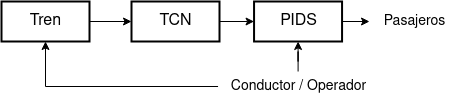
\includegraphics[width=0.66\textwidth]{./Figures/diagTrenTcnPids.png}
	\caption{Diagrama del sistema Tren-TCN-PIDS.}
	\label{fig:diagTrenTcnPids}
\end{figure}

La red TCN dispone define una comunicación usando dos buses jerárquicos llamados WTB y MVB. El sistema PIDS se interconecta al bus de datos MVB, como se indica en el diagrama de la figura \ref{fig:diagTcnPidsBuusesWtbMvb}.\\


\begin{figure}[ht]
	\centering
	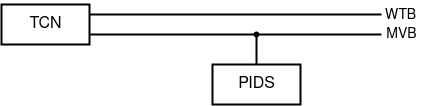
\includegraphics[width=0.66\textwidth]{./Figures/diagTcnPidsBusesWtbMvb.png}
	\caption{Diagrama de interconexión TCN-PIDS}
	\label{fig:diagTcnPidsBuusesWtbMvb}
\end{figure}

El sistema PIDS tiene un bus de comunicación propio a través de una red RS485. Uno de los componentes de esta red es el módulo SCU, al cual se conectan distintos dispositivos como los display LED, los mapas de recorrido LED, las cámaras y parlantes, tal como se indica en la figura 	\ref{fig:diagPidsScuDevices}.\\


\begin{figure}[ht]
	\centering
	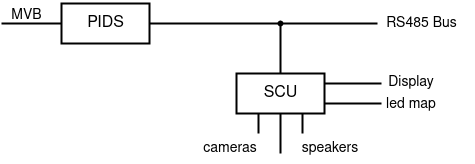
\includegraphics[width=0.66\textwidth]{./Figures/diagPidsScuDevices.png}
	\caption{Diagrama del módulo SCU en la red PIDS.}
	\label{fig:diagPidsScuDevices}
\end{figure}

Al módulo SCU se conectan las unidades IDU, que corresponden a los display LED de salón. Cada unidad IDU contiene un driver y el arreglo de módulos de matriz de led que conforman el display. En la figura \ref{fig:diagScuDriverDisplay} se representan estos bloques funcionales.\\


\begin{figure}[ht]
	\centering
	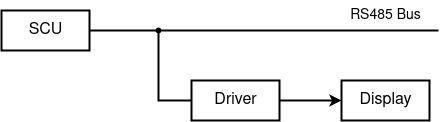
\includegraphics[width=0.66\textwidth]{./Figures/diagScuDriverDisplay.png}
	\caption{Diagrama de bloques del sistema SCU, placa de control y carteles LED de salón.}
	\label{fig:diagScuDriverDisplay}
\end{figure}

El alcance del sistema desarrollado en este trabajo cubre la funcionalidad de este conjunto de bloques Driver + Display, que en la nomenclatura del sistema PIDS existente corresponde a los módulos IDU. Existen dos unidades de estos módulos por cada salón. Comunmente un tren tiene siete salones, por lo que se tiene un mínimo de catorce unidades IDU más dos displays externos adicionales para el frente y contrafrente del tren que indican las estaciones cabecera del recorrido, dando un total aproximado de dieciséis unidades de control de display por cada tren.\\


\pagebreak
\subsection{Diseño}
La propuesta de diseño busca cubrir las funcionalidades del bloque de control del display LED. El display LED es una unidad que se puede adquirir comercialmente. Sin embargo el driver para la red PIDS es una solución propietaria del fabricante y es la que se busca reemplazar con este desarrollo.\\

En la figura \ref{fig:diagVistaReDisenhoEduCIAA} se presenta un diagrama de bloques del sistema de control propuesto. Este controlador usa comunicación serie a través de interfaces UART-RS485 y UART-USB. La UART es un periférico del microcontrolador de la plataforma CIAA. La alimentación de la CIAA difiere de aquella existente en la red RS485, por lo que también es necesario un bloque de conversión DC-DC para garantizar compatibilidad eléctrica. La comunicación con el display se realiza a través de un adaptador, que consiste básicamente en un puerto de entrada-salida.\\


\begin{figure}[ht]
	\centering
	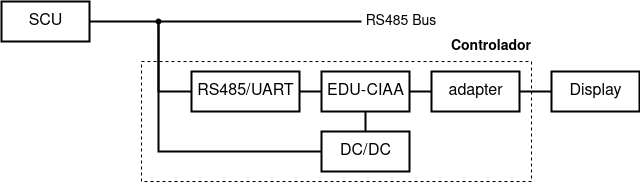
\includegraphics[width=0.75\textwidth]{./Figures/diagVistaReDisenhoEduCIAA.png}
	\caption{Diagrama de bloques del controlador propuesto.}
	\label{fig:diagVistaReDisenhoEduCIAA}
\end{figure}

A nivel lógico, el sistema que se propone consiste en cuatro objetos activos que interactúan entre sí, tal como se indica en la figura \ref{fig:diagVistaDisenho}. 

\begin{figure}[ht]
	\centering
	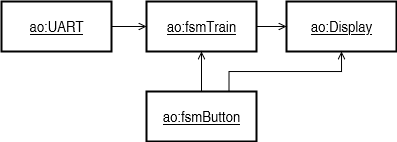
\includegraphics[width=0.75\textwidth]{./Figures/diagVistaDisenho.png}
	\caption{Vista de interacciones del sistema propuesto.}
	\label{fig:diagVistaDisenho}
\end{figure}

El objeto activo UART es el encargado de recibir e interpretar las tramas de datos que viajan por la red RS485 del bus de datos del SCU.

\begin{figure}[ht]
	\centering
	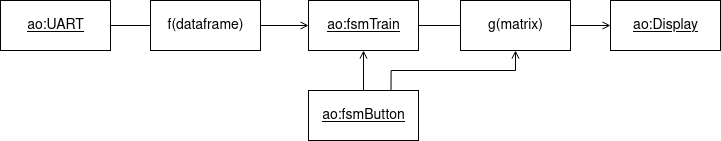
\includegraphics[width=1\textwidth]{./Figures/diagVistaDisenhoExtendida.png}
	\caption{Vista de interacciones extendida del sistema propuesto.}
	\label{fig:diagVistaDisenhoExtendida}
\end{figure}

\pagebreak
\subsection{Implementación}

El desarrollo de la arquitectura propuesta se basa en la interacción de máquinas de estado.
En este trabajo las máquinas de estado se implementan en C a partir de la siguiente estructura:

1. Definir los estados posibles con un tipo definido como "eSystemState":

\begin{lstlisting}[
	language=C, 
	backgroundcolor=\color{mygray},
	style=nonumbers]
typedef enum {
	STATE_INIT,
	STATE_LISTENING,
	STATE_HEADER,
	STATE_TRAILER
} eSystemState;
\end{lstlisting}

2. Definir los eventos que van a generar transiciones entre estados con un tipo definido "eSystemEvent":

\begin{lstlisting}[
	language=C, 
	backgroundcolor=\color{mygray},
	style=nonumbers]
typedef enum{
	evInit,
	evReceive,
	evHeader,
	evTrailer
} eSystemEvent;
\end{lstlisting}

3. A partir de un diagrama de la máquina de estados en cuestión, 
definir un tipo puntero a función definido como "*pfEventHandler()":

\begin{lstlisting}[
	language=C, 
	backgroundcolor=\color{mygray},
	style=nonumbers]
typedef eSystemState (*pfEventHandler)(void);
\end{lstlisting}

4: Definir una estructura para la máquina de estados con un tipo definido "sStateMachine" que incluya una variable estado (eSystemState), una variable evento (eSystemEvent) y un puntero a función (pfEventHandler). El puntero a función será una instancia de handler específico que maneje las transiciones entre estados. 

\begin{lstlisting}[
	language=C, 
	backgroundcolor=\color{mygray},
	style=nonumbers]
typedef struct{
	eSystemState 		fsmState;
	eSystemEvent 		fsmEvent;
	pfEventHandler 		fsmHandler;
} sStateMachine;
\end{lstlisting}

De esta manera queda desacoplada la implentación de los handlers del resto de la estructura de la máquina de estados, logrando portabilidad, escala y modularidad. Los handlers serán funciones que se implementan con el sufico Handler() y que por definición tienen un solo argumento de tipo void.

5. Definir los handlers a implementar para el manejo de ejecución y transiciones entre estados.

\begin{lstlisting}[
	language=C, 
	backgroundcolor=\color{mygray},
	style=nonumbers]

eSystemState 	InitHandler(void)		;
eSystemState 	ListeningHandler(void)	;
eSystemState 	HeaderHandler(void)		;
eSystemState 	TrailerHandler(void) 	;

\end{lstlisting}

Con esta técnica de desacoplamiento, se implementan dos archivos por cada máquina de estado : uno de encabezados (stateMachine.h) con las definiciones de los puntos 1 a 4 y otro con la implementación (stateMachine.c) de los handlers.

Una implementación de handler a modo de ejemplo se presenta a continuación.

\begin{lstlisting}[
	language=C, 
	backgroundcolor=\color{mygray},
	style=nonumbers]
eSystemState 	TrailerHandler(void){ 
	printf("STATE_TRAILER;\n");
	return STATE_LISTENING; 
}
\end{lstlisting}

6. Finalmente, cada implementación de máquina de estado debe definir la instancia de la máquina de estados propiamente dicha con un arreglo de estructuras definido como "sStateMachine fsmStateMachine []". Este arreglo de estructuras máquina de estados se define a partir de los estados, sus transiciones y los handlers correspondientes. En este punto es mandatorio incluir un diagrama de la máquina de estados.

\begin{lstlisting}[
	language=C, 
	backgroundcolor=\color{mygray},
	style=nonumbers]

sStateMachine fsmTest [] = 
{
	{STATE_INIT, evInit, InitHandler},
	{STATE_LISTENING, evReceive, ListeningHandler},
	{STATE_HEADER, evReceive, HeaderHandler},
	{STATE_TRAILER, evReceive, TrailerHandler}
};
\end{lstlisting}


El diagrama para esta máquina es el siguiente:

\begin{lstlisting}[
	language=C, 
	backgroundcolor=\color{mygray},
	style=nonumbers]
\end{lstlisting}


\begin{figure}[ht]
	\centering
	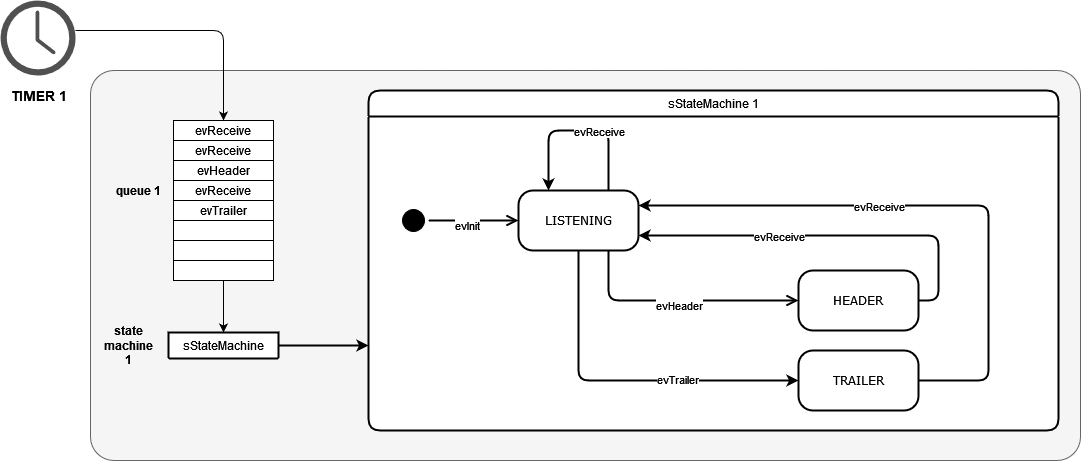
\includegraphics[width=1\textwidth]{./Figures/stateMachineUARTv1.png}
	\caption{Diagrama del objeto activo de la máquina de estados asociada.}
	\label{fig:fsmUARTv1}
\end{figure}

	
\pagebreak
\section{Patrones}



\begin{figure}[ht]
	\centering
	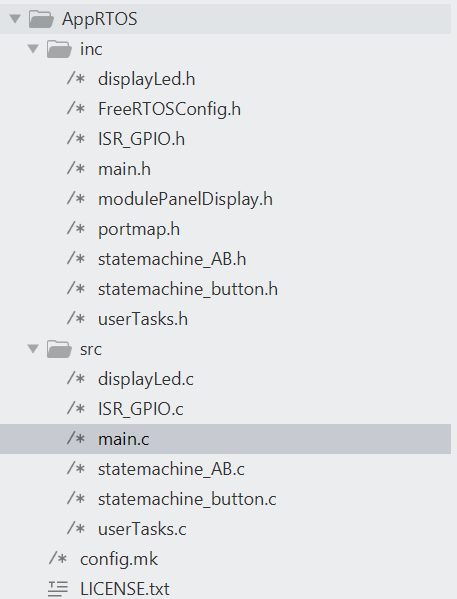
\includegraphics[width=1\textwidth]{./Figures/estructuraCodigos.png}
	\caption{Estructura del código en C.}
	\label{fig:codestructure}
\end{figure}

\begin{figure}[ht]
	\centering
	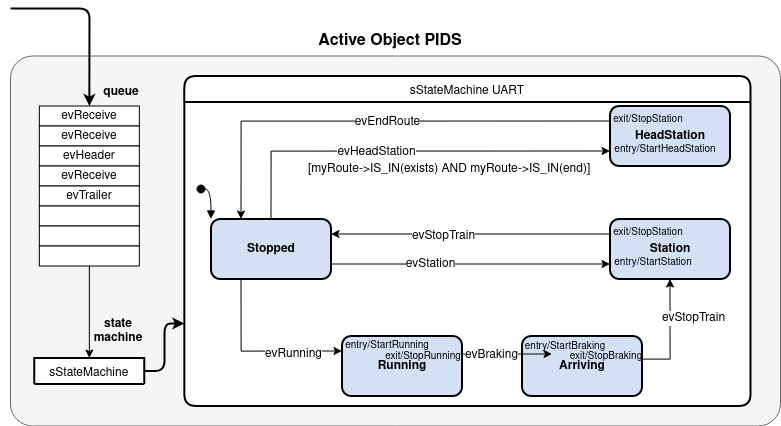
\includegraphics[width=1\textwidth]{./Figures/fsmTrain.png}
	\caption{Diagrama del objeto activo PIDS y detalle de la máquina de estados asociada.}
	\label{fig:fsmTrain}
\end{figure}

\pagebreak
\section{Firmware}


\begin{figure}[ht]
	\centering
	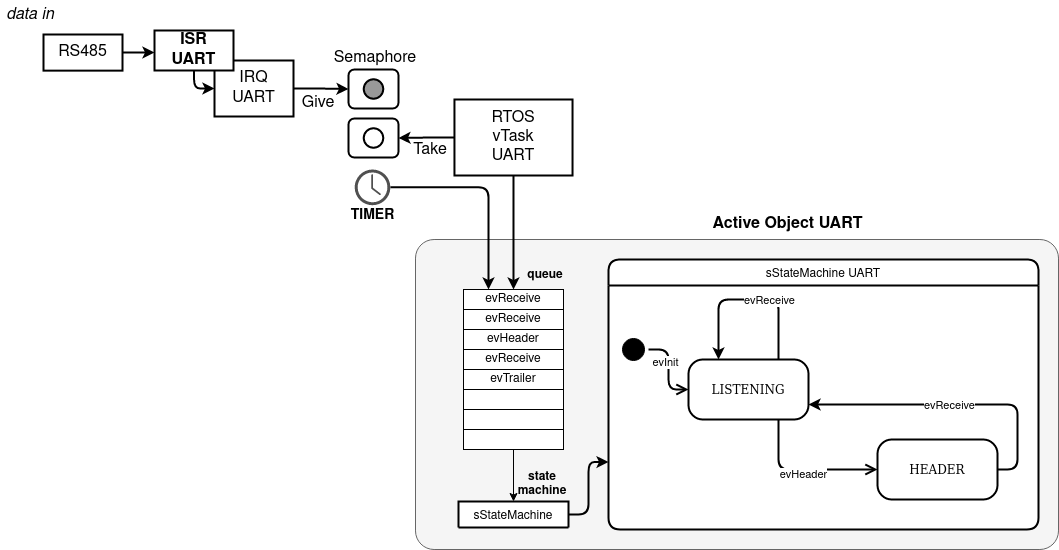
\includegraphics[width=1\textwidth]{./Figures/fsmUART.png}
	\caption{Diagrama de detalle de la implementación en RTOS del objeto activo UART.}
	\label{fig:fsmUART}
\end{figure}


\begin{figure}[ht]
	\centering
	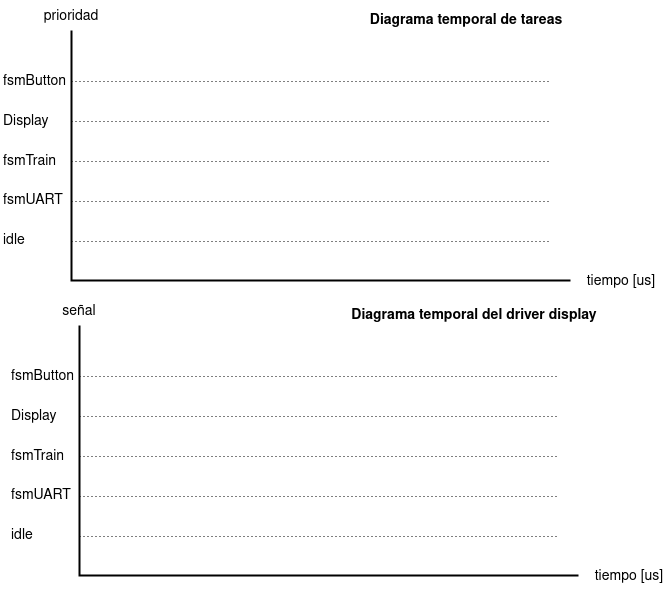
\includegraphics[width=1\textwidth]{./Figures/diagramasTemporales.png}
	\caption{}
	\label{fig:diagramasTemporales}
\end{figure}

\pagebreak
\section{Hardware}

\begin{figure}[ht]
	\centering
	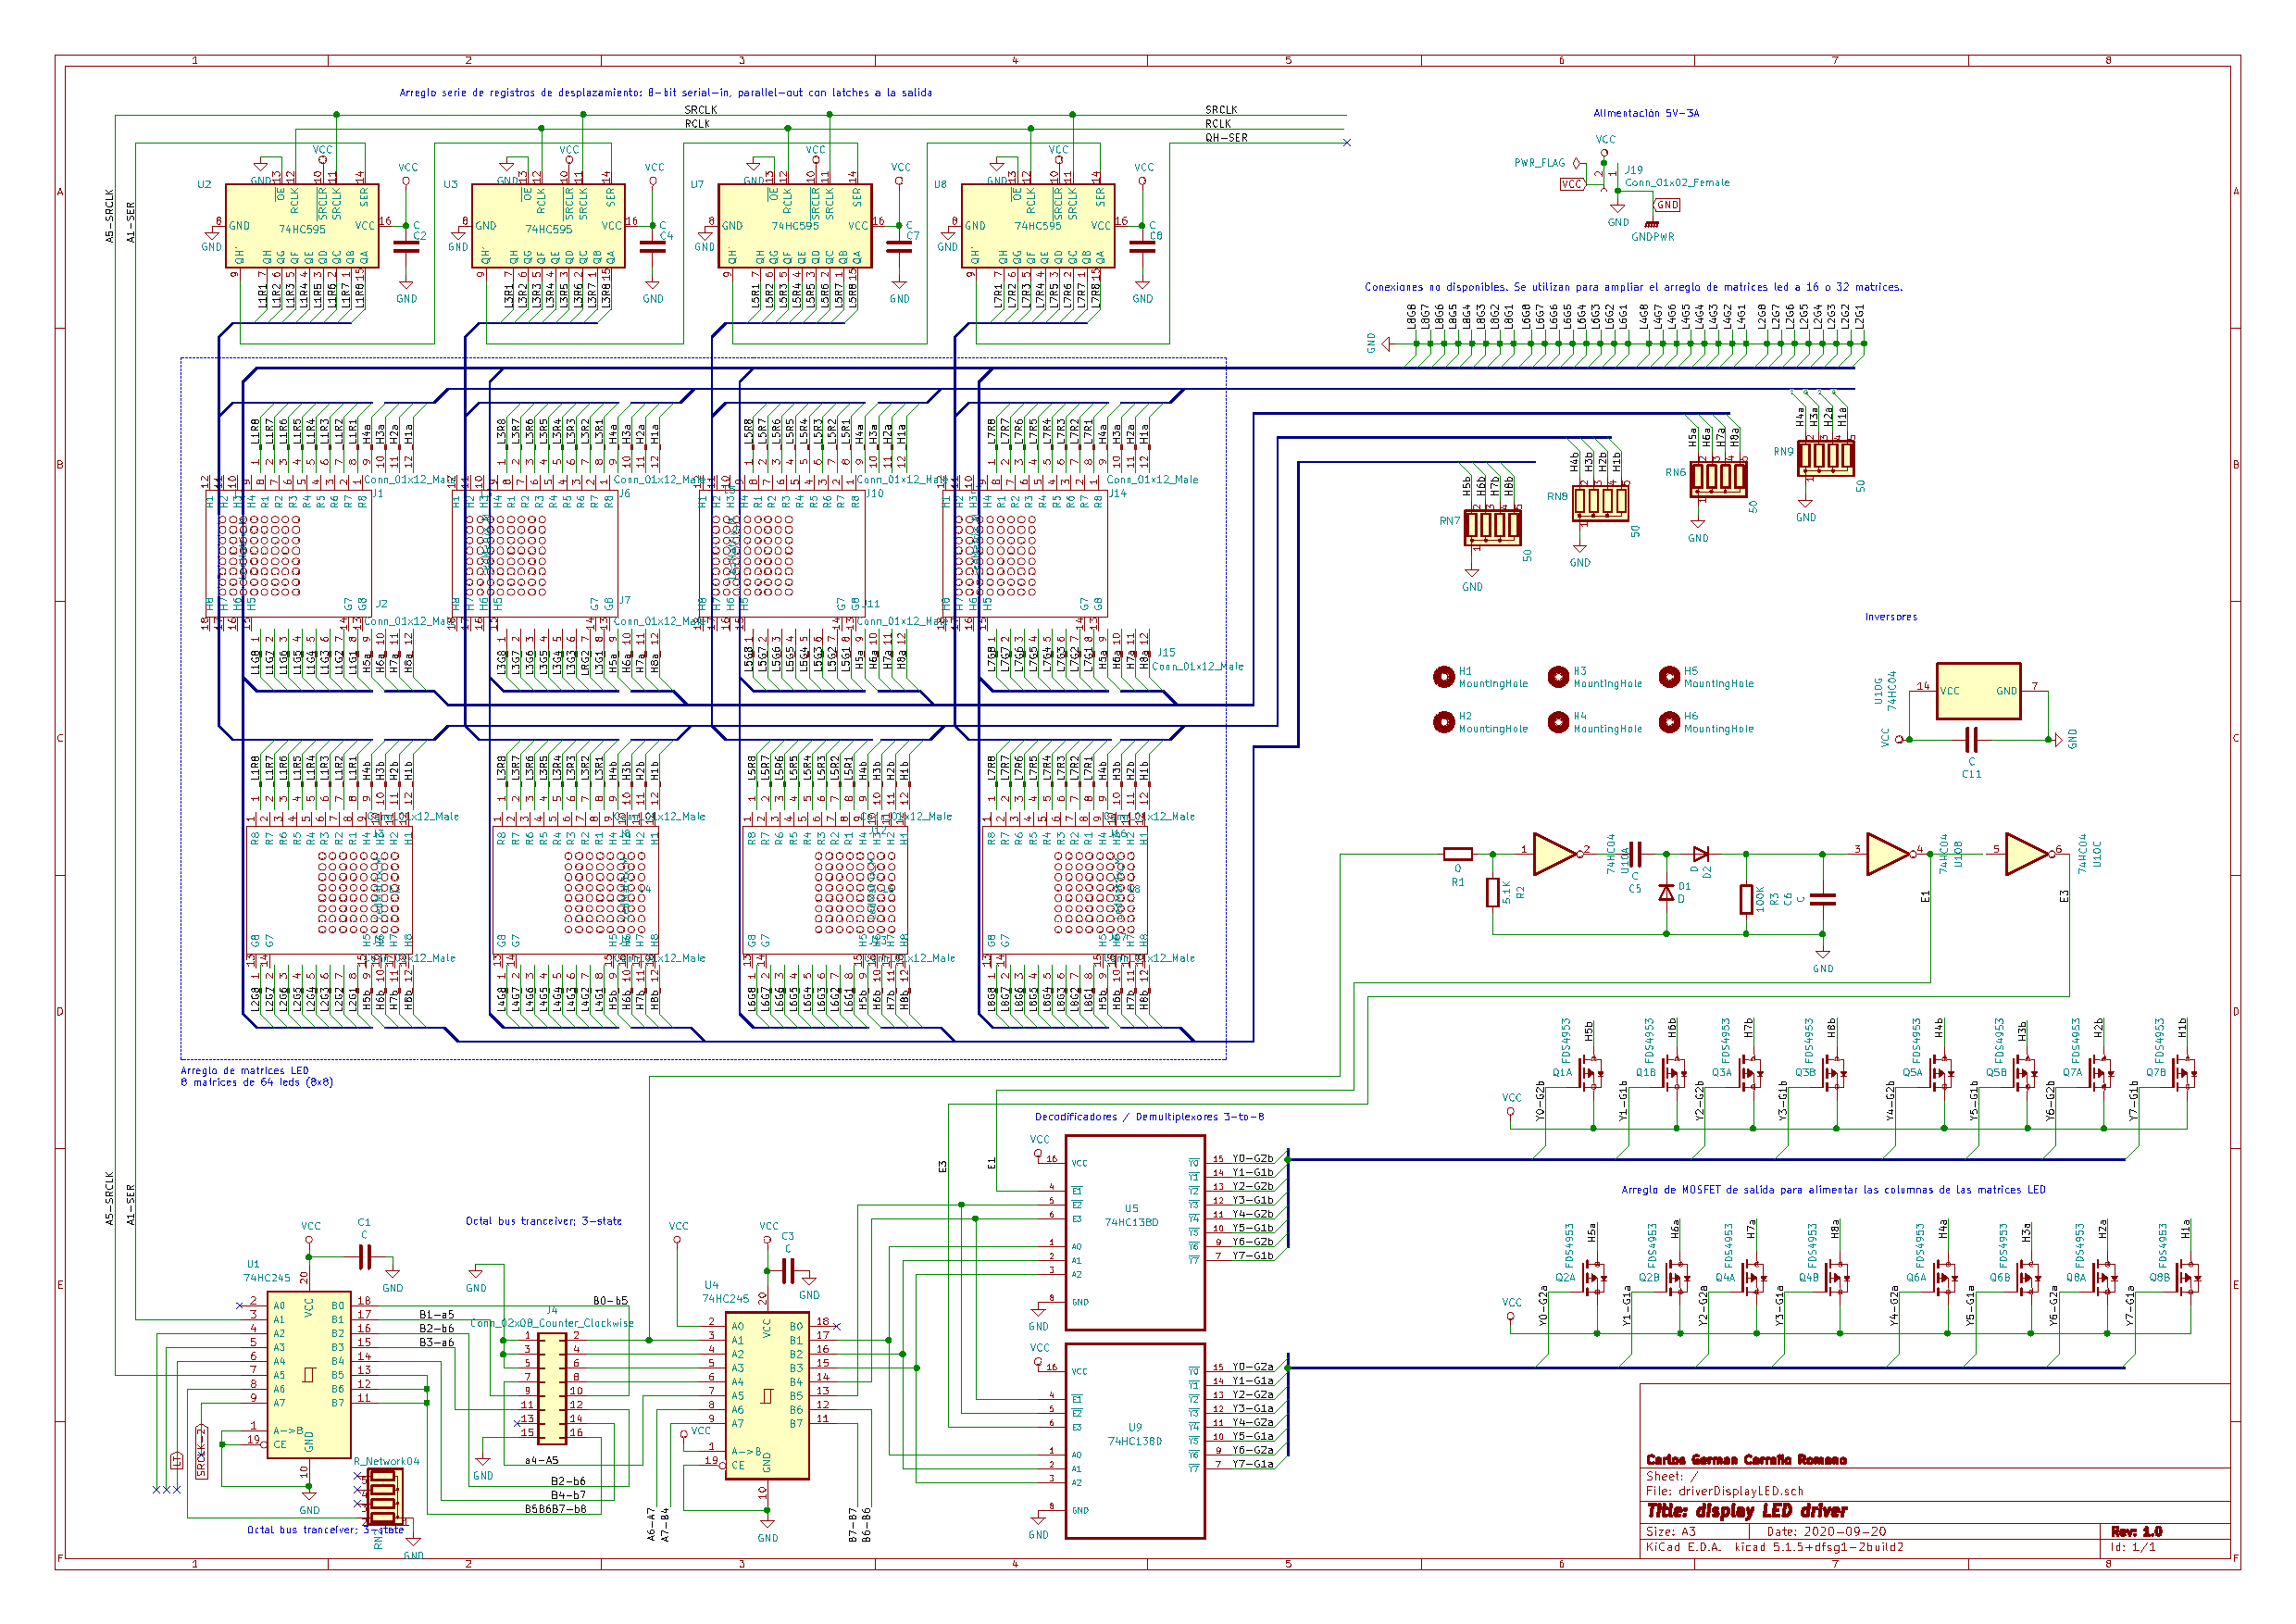
\includegraphics[width=1\textwidth]{./Figures/output.driverLED.pdf}
	\caption{Circuito esquemático de la placa driver de los carteles de matriz LED.}
	\label{fig:schDriverLED}
\end{figure}

\begin{figure}[ht]
	\centering
	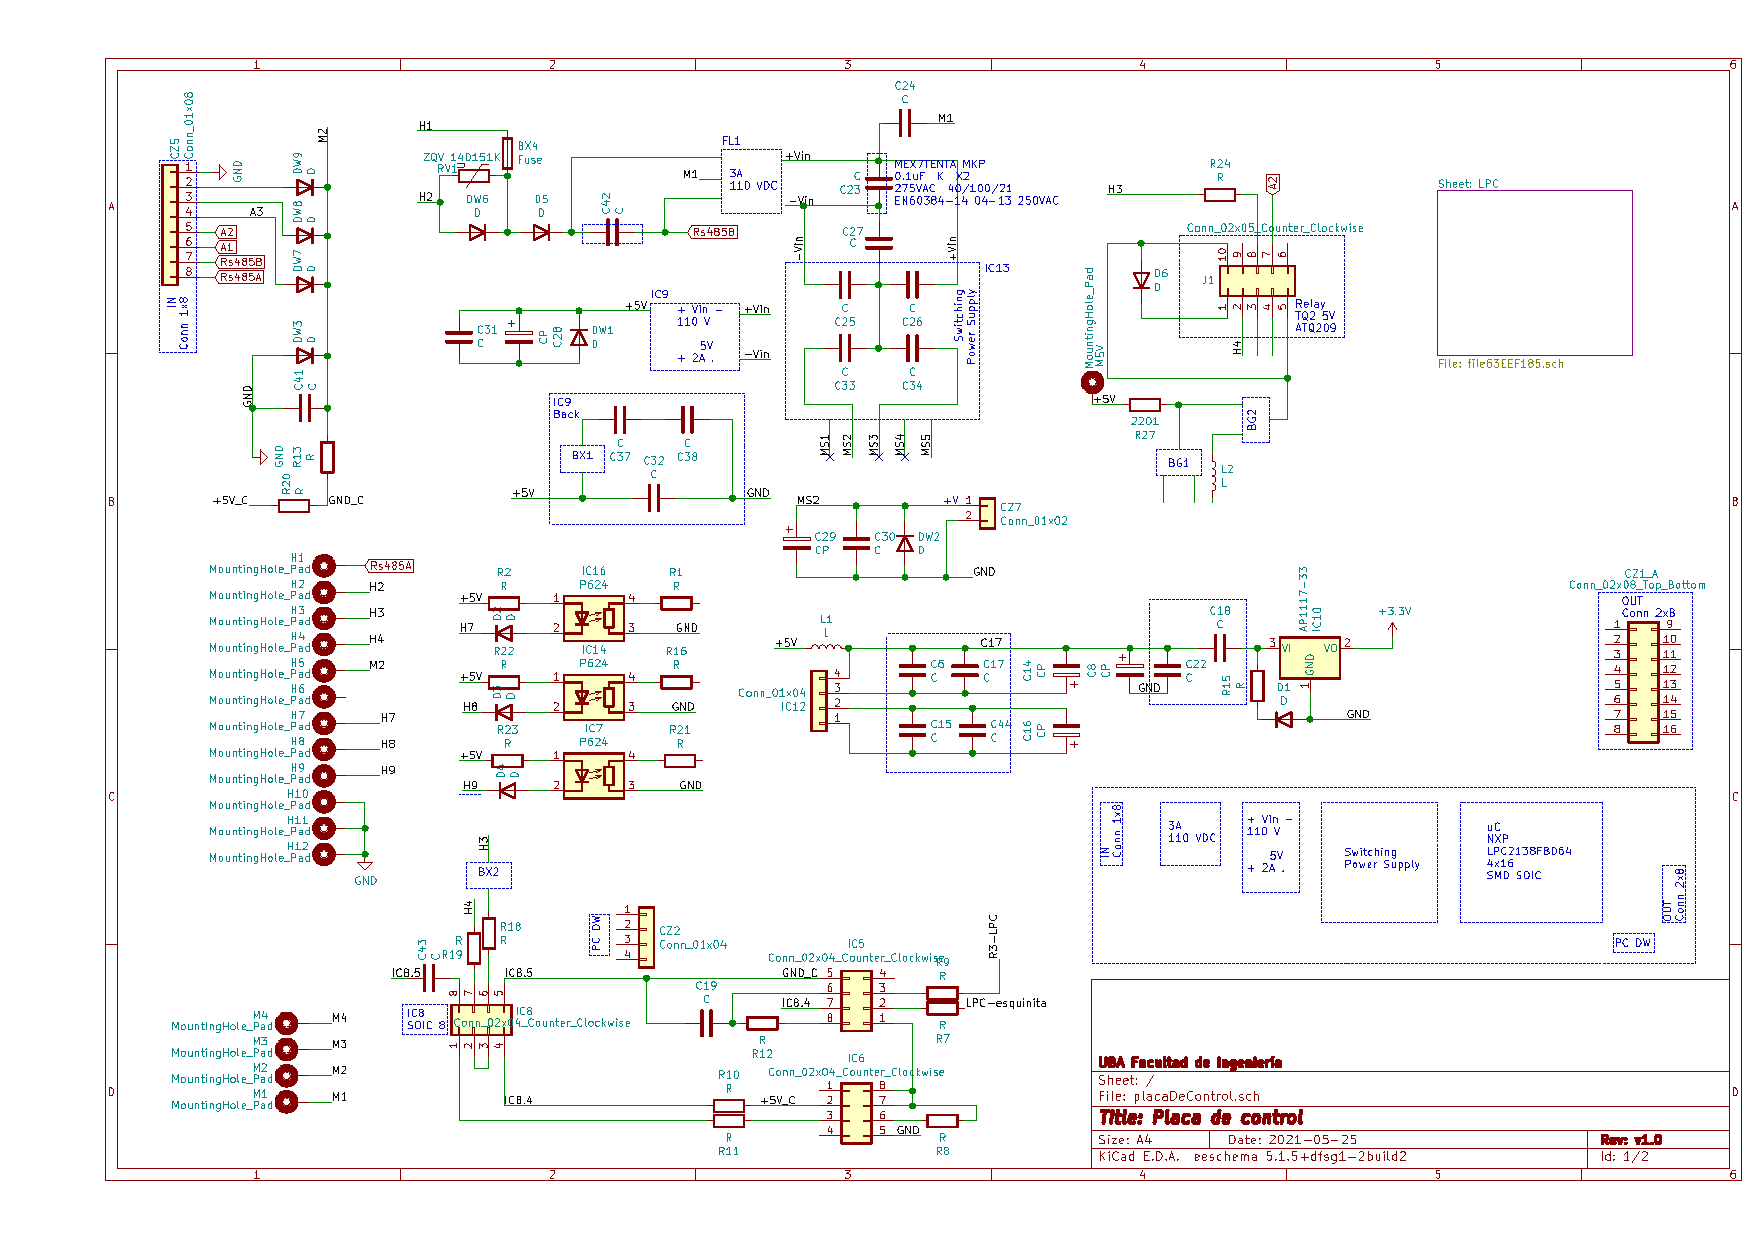
\includegraphics[width=1\textwidth]{./Figures/output.placaControl.pdf}
	\caption{Circuito esquemático de la placa de control de los carteles LED de salón.}
	\label{fig:schController}
\end{figure}

\begin{figure}[ht]
	\centering
	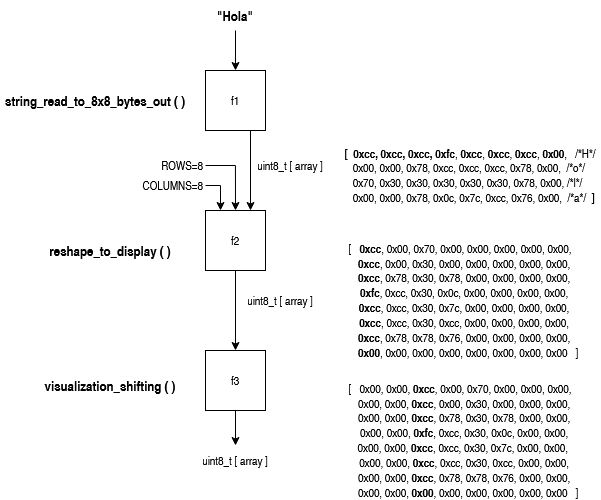
\includegraphics[width=1\textwidth]{./Figures/displayDataLogic.png}
	\caption{Lógica de procesamiento de datos para visualizar en el display.}
	\label{fig:displayDataLogic}
\end{figure}